\documentclass[tikz,border=5]{standalone}
\usepackage{amsmath,amssymb}
\usepackage{color}
\usepackage{tikz}
\usetikzlibrary{fadings}
\usetikzlibrary{patterns}
\usetikzlibrary{shadows.blur}
\usetikzlibrary{shapes}

\begin{document}

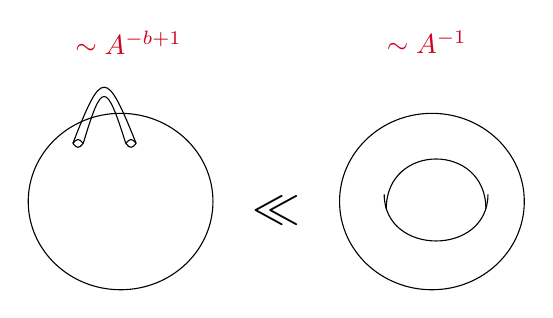
\begin{tikzpicture}[x=0.75pt,y=0.75pt,yscale=-1,xscale=1]


\draw  %circle
(28.5,53.5) .. controls (28.5,30.03) and (48.43,11) .. (73,11) .. controls (97.58,11) and (117.5,30.03) .. (117.5,53.5) .. controls (117.5,76.97) and (97.58,96) .. (73,96) .. controls (48.43,96) and (28.5,76.97) .. (28.5,53.5) -- cycle ;
\draw %thin tube lower curve
(50,25.5) .. controls (64,-10.56) and (66,-10.69) .. (80.5,25.5) ;
\draw %thin tube upper curve
(55,25.5) .. controls (64,-4.56) and (66,-4.69) .. (75.5,25.5) ;
\draw  %thin tube
(50,25.5) .. controls (52,23) and (53,23) .. (55,25.5) ;
\draw  %thin tube
(50,25.5) .. controls (52,28) and (53,28) .. (55,25.5) ;
\draw  %thin tube right circle
(75.5,25.5) .. controls (77.5,23) and (78.5,23) .. (80.5,25.5) ;
\draw  %thin tube right circle
(75.5,25.5) .. controls (77.5,28) and (78.5,28) .. (80.5,25.5) ;


\draw  %circle
(178.5,53.5) .. controls (178.5,30.03) and (198.43,11) .. (223,11) .. controls (247.58,11) and (267.5,30.03) .. (267.5,53.5) .. controls (267.5,76.97) and (247.58,96) .. (223,96) .. controls (198.43,96) and (178.5,76.97) .. (178.5,53.5) -- cycle ;
\draw %torus
(200,50) .. controls (200,80) and (250,80) .. (250,50) ;
\draw %torus
(201,57) .. controls (201,25) and (249,25) .. (249,57) ;

% Text Node
\draw (135.5,50) node [anchor=north west][inner sep=0.75pt]  [rotate=0] [align=left] {{\fontsize{18pt}{18pt}\selectfont $\ll$}};%
% Text Node
% Text Node
 \draw (200,-30) node [anchor=north west][inner sep=0.75pt]    {$\textcolor[rgb]{0.82,0.01,0.11}{\sim A^{-1}}$};
% Text Node
 \draw (50,-30) node [anchor=north west][inner sep=0.75pt]    {$\textcolor[rgb]{0.82,0.01,0.11}{\sim A^{-b+1}}$};

\end{tikzpicture}

\end{document}